%% Time-stamp: Mon Jun 17 12:30:17 2013
\chapter{First order differential Equations}
\label{cha:diffeqs}

\section{What is a Differential Equation?} %{{{1
\label{sec:what-diffeq}
A \emph{differential equation} is an equation involving an unknown function and its
derivatives.  A general differential equation can contain second derivatives and
higher derivatives of the unknown function, but in this course we will only consider
differential equations that contain first order derivatives.  So the most general
differential equation we will look at is of the form
\begin{equation}
  \frac{\dd y}{ \dd x} = f(x, y).
  \label{eq:mother-of-all-diffeqs}
\end{equation}
Here $f(x,y)$ is any expression that involves both quantities $x$ and $y$.  For
instance, if $f(x,y) = x^2+y^2$ then the differential equation represented by
\eqref{eq:mother-of-all-diffeqs} is
\[
  \frac{\dd y}{\dd x} = x^2 + y^2.
\]
In this equation $x$ is a variable, while $y$ is a function of $x$.

Differential equations appear in many science and engineering problems, as we will
see in the section on applications.  But first let's think of a differential equation
as a purely mathematical question: \textit{which functions $y=y(x)$ satisfy the
  equation \eqref{eq:mother-of-all-diffeqs}?}  It turns out that there is no general
method that will always give us the answer to this question, but there are methods
that work for certain special kinds of differential equations.  To explain all this,
this chapter is divided into the following parts:
\begin{itemize}
\item Some basic examples that give us a clue as to what the solution to a general
  differential equation will look like.
\item Two special kinds of differential equation (``separable'' and ``linear''), and
  how to solve them.
\item How to visualize the solution of a differential equation (using ``direction
  fields'') and how to compute the solution with a computer using Euler's method.
\item Applications: a number of examples of how differential equations come up and
  what their solutions mean.
\end{itemize}

\section{Two basic examples} %{{{1

\subsection{Equations where the RHS does not contain $y$} %{{{2
\label{sec:diffeq-y-missing}

Which functions $y=y(x)$ satisfy
\begin{equation}
  \label{eq:diffeq-example-y-missing}
  \frac{\dd y} {\dd x} = \sin x ~?
\end{equation}
This is a differential equation of the form~\eqref{eq:mother-of-all-diffeqs} where
the function $f$ that describes the Right Hand Side is given by $f(x,y) = \sin x$.
In this example the function $f$ does not depend on the unknown function $y$.
Because of this the differential equation really asks ``\textit{which functions of
  $x$ have $\sin x$ as derivative?}''  In other words, which functions are the
antiderivative of $\sin x$?  We know the answer, namely
\[
y = \int \sin x\;\dd x = -\cos x +C
\]
where $C$ is an arbitrary constant.
This is the solution to the differential
equation~\eqref{eq:diffeq-example-y-missing}.  This example shows us that there
is not just one solution, but that there are many solutions.  The expression
that describes \emph{all solutions} to the differential equation
\eqref{eq:diffeq-example-y-missing} is called \emph{the general solution}.  It
contains an unknown constant $C$ that is allowed to have arbitrary values.

To give meaning to the constant $C$ we can observe that when $x=0$ we have
\[
y(0) = - \cos 0 + C = -1+C.
\]
So the constant $C$ is nothing but
\[
C=y(0)+1.
\]
For instance, the solution of~\eqref{eq:diffeq-example-y-missing} that also satisfies
$y(0)=4$ has $C=4+1=5$, and thus is given by
\[
y(x) = -\cos x + 5.
\]
We have found that there are many solutions to the differential
equation~\eqref{eq:diffeq-example-y-missing} (because of the undetermined constant
$C$), but as soon as we prescribe the value of the solution for one value of $x$,
such as $x=0$, then there is exactly one solution (because we can compute the
constant $C$.)


\subsection{The exponential growth example} %{{{2
\textit{Which functions equal their own derivative}, i.e.~which functions satisfy
\[
\frac{\dd y} {\dd x} = y ~?
\]
Everyone knows at least one example, namely $y=e^x$.  But there are more solutions:
the function $y=0$ also is its own derivative.  From the section on exponential
growth in math 221 we know all solutions to $\frac{\dd y} {\dd x} = y$.  They are
given by
\[
y(x) = C e^x,
\]
where $C$ can be an arbitrary number.  If we know the solution $y(x)$ for some value
of $x$, such as $x=0$, then we can find $C$ by setting $x=0$:
\[
y(0) = C.
\]
Again we see that instead of there being one solution, the general solution contains
an arbitrary constant $C$.

\subsection{Summary} %{{{2
\label{sec:summary-1}
The two examples that we have just seen show us that for certain differential
equations
\begin{itemize}
\item there are many solutions,
\item the formula for the general solution contains an undetermined constant $C$,
\item the undetermined constant $C$ becomes determined once we specify the value of
  the solution $y$ at one particular value of $x$.
\end{itemize}
It turns out that these features are found in almost all differential equations of
the form~\eqref{eq:mother-of-all-diffeqs}.  In the next two sections we will see
methods for computing the general solution to two frequently occurring kinds of
differential equation, the \textit{separable equations}, and the \textit{linear
  equations.}

\section{First Order Separable Equations} %{{{1
\label{sec:1storder-separable}
By definition a \emph{separable differential equation} is a diffeq of the form
\begin{equation}
  \label{eq:separable-2}
  y'(x) = F(x) G(y(x)),\quad\text{or}\quad \frac{\dd y}{\dd x} = F(x)G(y).
\end{equation}
Thus the function $f(x,y)$ on the right hand side in
\eqref{eq:mother-of-all-diffeqs} has the special form
\[
  f(x,y) = F(x)\, G(y).
\]
For example, the differential equation 
\[
  \frac{\dd y}{\dd x} = \sin(x) \bigl(1+y^2\bigr)
\]
is separable, and one has $F(x) = \sin x$ and $G(y) = 1+y^2$.
On the other hand, the differential equation
\[
  \frac{\dd y}{\dd x} = x+y
\]
is not separable.

\subsection{Solution method for separable equations} %{{{2
To solve this equation divide by $G(y(x))$ to get
\begin{equation}
  \label{eq:separated}
  \frac{1}{ G(y(x))} \frac{\dd y}{\dd x} = F(x). 
\end{equation}
Next find a function $H(y)$ whose derivative with respect to $y$ is
\begin{equation}\label{eq:separable-3}
  H'(y) = \frac{1}{G(y)}
  \quad\left(\text{solution: } H(y) = \int {\frac{dy}{G(y)}}.\right)
\end{equation}
Then the chain rule implies that the left hand side in (\ref{eq:separated}) can be written as
\[
  \frac{1}{ G(y(x))} \frac{\dd y}{\dd x} = H'(y(x)) \frac{\dd y}{\dd x} =
  \frac{\dd H(y(x))}{\dd x}.
\]
Thus \eqref{eq:separated} is equivalent with
\[
\frac{\dd H(y(x))}{\dd x} = F(x).
\]
In words: $H(y(x))$ is an antiderivative of $F(x)$, which means we can find $H(y(x))$
by integrating $F(x)$:
\begin{equation}
  \label{eq:separable-solution}
  H(y(x)) = \int F(x) dx +C. 
\end{equation}
Once we have found the integral of $F(x)$ this gives us $y(x)$ in implicit form: the
equation (\ref{eq:separable-solution}) gives us $y(x)$ as an \textit{implicit
  function} of $x$.  To get $y(x)$ itself we must solve the equation
(\ref{eq:separable-solution}) for $y(x)$.

A quick way of organizing the calculation goes like this:
\begin{quote}
  To solve \(\DS\frac{\dd y}{\dd x} = F(x)G(y)\) we first \textit{separate the
    variables},
  \[
  \frac{\dd y}{G(y)} = F(x)\,\dd x,
  \]
  and then integrate,
  \[
  \int\frac{\dd y}{G(y)} = \int F(x)\,\dd x.
  \]
  The result is an implicit equation for the solution $y$ with one undetermined
  integration constant.
\end{quote}

\subsubsection*{Determining the constant} The solution we get from the above
procedure contains an arbitrary constant $C$. If the value of the solution is
specified at some given $x_0$, i.e. if $y(x_0)$ is known then we can express $C$ in
terms of $y(x_0)$ by using (\ref{eq:separable-solution}).

\subsection{A snag: }\label{sec:snag} We have to divide by $G(y)$ which is %{{{2
problematic when $G(y)=0$. This has as consequence that in addition to the solutions
we found with the above procedure, there are at least a few more solutions: the
zeroes of $G(y)$ (see Example \ref{ex:snag} below). In addition to the zeroes of
$G(y)$ there sometimes can be more solutions, as we will see in Example
\ref{ex:leakybucket} on ``Leaky Bucket Dating.''

\subsection{Example} %{{{2
We solve
\[
\frac{\dd z}{\dd t} = (1+z^2)\cos t.
\]
Separate variables and integrate
\[
\int\frac{\dd z}{1+z^2} = \int\cos t\,\dd t,
\]
to get
\[
\arctan z = \sin t +C.
\]
Finally solve for $z$ and we find the general solution
\[
z(t) = \tan \bigl (\sin (t) +C\bigr).
\]

\subsection{Example: the snag in action}\label{ex:snag} %{{{2
If we apply the method to $y'(x)=y$, we get
\[
y(x) = e^{x+C}.
\]
No matter how we choose $C$ we never get the function $y(x)=0$, even though $y(x)=0$
satisfies the equation.  This is because here $G(y)= y$, and $G(y)$ vanishes for
$y=0$.

\section{Problems} %{{{1
\problemfont %{{{3
\begin{multicols}{2}
For each of the following differential equations
\begin{trivlist}
\item [-] find the general solution,
\item [-] indicate which, if any, solutions were lost while separating variables,
\item [-] find the solution that satisfies the indicated initial values.
\end{trivlist}

\problem $\DS \frac{\dd y} {\dd x} = xy$, \quad $y(2) = -1$. %{{{3

\answer %{{{3
General solution $y(x) = Ce^{\frac12 x^2}$; initial conditions imply $C=-e^{-2}$.  
\endanswer

\problem \(\DS \frac{\dd y}{\dd x} + x\cos^2y =0,\quad y(0)=\tfrac\pi3.  \) %{{{3

\answer %{{{3
Implicit form of the solution $\tan y = -\frac{x^2}{2}+C$, so $C=
\tan\pi/3 = \sqrt3$.

Solution $y(x) = \arctan\bigl(\sqrt3 - x^2/3\bigr)$
\endanswer

\problem \(\DS \frac{\dd y}{\dd x} + \frac{1+x}{1+y} =0,\quad y(0)=A.  \) %{{{3

\answer %{{{3
Implicit form of the solution: $y+\frac12y^2 +x+\tfrac12x^2 =
A+\tfrac12A^2$.  If we solve for $y$ we get
\[
y = -1\pm \sqrt{A^2+2A+1-x^2-2x}
\]
Whether we need the ``$+$'' or ``$-$'' depends on $A$.
\endanswer


\problem \(\DS y^2\frac{\dd y}{\dd x} + x^3 =0, y(0)=A.  \) %{{{3

\answer %{{{3
Implicit form of the solution $\frac13y^3+\frac14x^4 = C$;
$C=\frac{1}{3}A^3$.  Solution is $y = \sqrt[3]{A^3-\frac34 x^4}$.
\endanswer

\problem \(\DS \frac{\dd y}{\dd x} + 1 - y^2 =0,\quad y(0)=A.  \) %{{{3

\answer %{{{3
Integration gives $\DS \frac12\ln\left|\frac{y-1}{y+1}\right| = x+C$.
Solve for $y$ to get $\frac{y-1}{y+1} = \pm e^{2x+2C} = \bigl(\pm
e^{2C}\bigr)e^{2x}$.

Let $B= \pm e^{2C}$ be the new constant and we get $\dfrac{y-1}{y+1} =
Be^{2x}$ whence $y = \dfrac{1+Be^{2x}}{1-Be^{2x}}$.

The initial value $y(0)=A$ tells us that $B = \frac{A-1}{A+1}$, and
therefore the solution with initial value $y(0) = A$ is $y =
\dfrac{A+1 + (A-1)e^{2x}}{A+1-(A-1)e^{2x}}$.
\endanswer

\problem \(\DS \frac{\dd y}{\dd x} + 1 + y^2 =0,\quad y(0)=A.  \) %{{{3

\answer %{{{3
$y(x) = \tan\bigl(\arctan (A) - x\bigr)$.
\endanswer


\problem $\DS\frac{\dd y}{\dd x}+\frac{x^2-1}{y}=0$,\quad $y(0)=1$. %{{{3

\answer  %{{{3
$y=\sqrt{2(x-\frac{x^3}3)+1}$
\endanswer

\problem\groupproblem% %{{{3
Let $P(t)$ be the size of a colony of bacteria in a Petri dish in some
experiment.  Assume that the size of the colony changes according to the
so-called logistic equation:
\[
\frac{\dd P} {\dd t} = \frac{1} {50} P(1000-P),
\]
Assume also that in the beginning of the experiment the population size is $P=100$.

\subprob Find the general solution to the differential equation.

\subprob Find the solution that satisfies the given initial conditions.

\subprob How long does it take the population to reach size $P=500$?

\subprob How long does it take the population to reach size $P=900$?

\subprob What value does $P$ have when $\frac{\dd P} {\dd t}$ is the largest (hint:
you do not need to solve the differential equation--this question has a very short
answer.)

\end{multicols}
\noproblemfont

\section{First Order Linear Equations} %{{{1
\label{sec:1storder-linear}
Differential equations of the form equation
\begin{equation}
  \frac{\dd y}{\dd x}+a(x)y = k(x)
  \label{eq:inhomogeneous-linear}
\end{equation}
are called \emph{first order linear}.  

\subsection{The Integrating Factor} %{{{2
\label{sec:integrating-factor}
Linear equations can always be solved by multiplying both sides of the equation
with a specially chosen function called the \emph{integrating factor.}  It is
defined by
\begin{equation}
  A (x) = \int a(x)\,\dd x,\qquad m (x) = e^{A (x)}.
  \label{eq:integrating-factor-defined}
\end{equation}
Here $m(x)$ is the integrating factor.  It looks like we just pulled this definition
of $A(x)$ and $m(x)$ out of a hat.  The example in \S~\ref{sec:an-example} shows
another way of finding the integrating factor, but for now let's go on with these two
functions.

Multiply the equation~\eqref{eq:inhomogeneous-linear} by the integrating factor
$m(x)$ to get
\[
m(x)\frac{\dd y}{\dd x}+a(x)m(x)y = m(x)k(x).
\]
By the chain rule the integrating factor satisfies
\[
\frac{\dd m(x)}{\dd x} = \frac{\dd\,
  e^{A(x)}} {\dd x}
= \underbrace{A'(x)}_{=a(x)} ~\underbrace{e^{A(x)}_{}}_{=m(x)}
= a(x)m(x).
\]
Therefore one has
\begin{align*}
  \frac{\dd m(x)y}{\dd x}
  &= m(x)\frac{\dd y}{\dd x}+a(x)m(x)y \\
  &= m(x)\Bigl\{\frac{\dd y}{\dd x}+a(x)y \Bigr\}\\
  &= m(x)k(x).
\end{align*}
Integrating and then dividing by the integrating factor gives the solution
\[
y=\frac1{m(x)}\left(\int m(x)k(x)\,\dd x+C\right).
\]
In this derivation we have to divide by $m(x)$, but since $m(x)=e^{A (x)}$ and since
exponentials never vanish we know that $m (x)\neq0$, so we can always divide by $m
(x)$.


\subsection{An example} %{{{2
\label{sec:an-example}\itshape%
Find the general solution to the differential equation
\[
\frac{\dd y} {\dd x} = y + x.
\]
Then find the solution that satisfies \upshape
\begin{equation}
  y(2)=0.
  \label{eq:example-linear-initial-condition}
\end{equation}
\subsubsection*{Solution}
We first write the equation in the standard linear form
\begin{equation}
  \label{eq:diffeq-linear-example}
  \frac{\dd y} {\dd x} - y = x,
\end{equation}
and then multiply with the integrating factor $m(x)$.  We could of course memorize
the formulas \eqref{eq:integrating-factor-defined} that lead to the integrating
factor, but a safer approach is to remember the following procedure, which will
always give us the integrating factor.

Assuming that $m(x)$ is as yet unknown we multiply the differential
equation~\eqref{eq:diffeq-linear-example} with $m$,
\begin{equation}
  m(x)\frac{\dd y} {\dd x} - m(x) y = m(x)x.
  \label{eq:example-multiplied-with-m}
\end{equation}
If $m(x)$ is such that
\begin{equation}
  -m(x) = \frac{\dd m(x)} {\dd x},
  \label{eq:integrating-factor-condition}
\end{equation}
then equation~\eqref{eq:example-multiplied-with-m} implies
\[
  m(x)\frac{\dd y} {\dd x} + \frac{\dd m(x)} {\dd x} y = m(x)x.
\]
The expression on the left is exactly what comes out of the product rule -- this is
the point of multiplying with $m(x)$ and then insisting
on~\eqref{eq:integrating-factor-condition}.  So, if $m(x)$
satisfies~\eqref{eq:integrating-factor-condition}, then the differential equation for
$y$ is equivalent with
\[
\frac{\dd m(x) y} {\dd x} = m(x) x.
\]
We can integrate this equation,
\[
m(x) y = \int m(x) x \;\dd x,
\]
and thus find the solution
\begin{equation}
  y(x) =  \frac{1} {m(x)}  \int m(x) x \;\dd x.
  \label{eq:example-linear-almost-solved}
\end{equation}
All we have to do is find the integrating factor $m$.  This factor can be any
function that satisfies~\eqref{eq:integrating-factor-condition}.
Equation~\eqref{eq:integrating-factor-condition} is a differential equation for $m$,
but it is separable, and we can easily solve it:
\[
\frac{\dd m} {\dd x} = -m \iff
\frac{\dd m} {m} = -\dd x \iff
\ln|m| = -x +C.
\]
Since \textit{we only need one integrating factor} $m$ we are not interested in
finding all solutions of~\eqref{eq:integrating-factor-condition}, and therefore we
can choose the constant $C$.  The simplest choice is $C=0$, which leads to
\[
\ln |m| = -x \iff |m| = e^{-x} \iff m = \pm e^{-x}. 
\]
Again, we only need one integrating factor, so we may choose the $\pm$~sign: the simplest
choice for $m$ here is
\[
m(x) = e^{-x}.
\]
With this choice of integrating factor we can now complete the calculation that led
to~\eqref{eq:example-linear-almost-solved}.  The solution to the differential
equation is
\begin{align*}
  y(x)
  &= \frac{1} {m(x)}  \int m(x) x \;\dd x \\
  &= \frac{1} {e^{-x}} \int e^{-x}x \;\dd x
  &\text{\color{badgerred}\sffamily\footnotesize%
    (integrate by parts)}\\
  &= e^{x} \Bigl\{-e^{-x}x - e^{-x} + C\Bigr\} \\
  &= -x-1+Ce^x.
\end{align*}
This is the general solution.

To find the solution that satisfies not just the differential equation, but also the
``initial condition''~\eqref{eq:example-linear-initial-condition}, i.e.~$y(2)=0$, we
compute $y(2)$ for the general solution,
\[
y(2) = -2-1+Ce^2 = -3 + Ce^2.
\]
The requirement $y(2) = 0$ then tells us that $C=3e^{-2}$.  The solution of the
differential equation that satisfies the prescribed initial condition is therefore
\[
y(x) = -x-1+3e^{x-2}.
\]

\section{Problems} %{{{1
\problemfont %{{{3
\begin{multicols}{2}

\problem In example~\ref{sec:an-example} we needed a function $m(x)$ that %{{{3
satisfies~\eqref{eq:integrating-factor-condition}.  The function $m(x) = 0$ satisfies
that equation. Why did we not choose $m(x)=0$?

\problem Why can't we simplify the computation at the end in %{{{3
example~\ref{sec:an-example} by canceling the two factors $m(x)$ as follows:
\begin{align*}
 y(x)
  &= \frac{1} {\cancel{m(x)}}  \int \cancel{m(x)}~ x \;\dd x \\
  &= \int x\;\dd x\\
  &= \frac12 x^2 + C?
\end{align*}

\centerline{\rule{1in}{1pt}}

For each of the following differential equations
\begin{trivlist}\itshape
\item[-] specify the differential equation that the integrating factor satisfies,
\item[-] find one integrating factor,
\item[-] find the general solution,
\item[-] find the solution that satisfies the specified initial conditions.
\end{trivlist}
In these problems $K$ and $N$ are constants.

\problem $\DS \frac{\dd y} {\dd x} = -y + x$,\quad $y(0)=0$. %{{{3

\problem $\DS \frac{\dd y} {\dd x} = 2y + x^2$,\quad $y(0)=0$. %{{{3

\problem \(\DS \frac{\dd y}{\dd x}+2y+ e^x = 0 \). %{{{3
\answer  %{{{3
$y=Ce^{-2x}-\frac13 e^x$
\endanswer

\problem \(\DS \frac{\dd y}{\dd x} - (\cos x)y = e^{\sin x}, y(0)=A.  \) %{{{3
\answer %{{{3
$y=xe^{\sin x}+Ae^{\sin x}$
\endanswer

\problem $\DS \frac{\dd y} {\dd x} = -10y + e^{-x}$,\quad $y(0)=0$. %{{{3

\problem $\DS \frac{\dd y} {\dd x} =y \tan x + 1$,\quad $y(0)=0$. %{{{3
\answer %{{{3
$m(x) = \cos x$, $\DS y(x) = \tan x + \frac{C} {\cos x}$, $C=0$.
\endanswer

\problem $\DS \frac{\dd y} {\dd x} = -y\tan x + 1$,\quad $y(0)=0$. %{{{3
\answer %{{{3
$\DS m(x) = \frac{1} {\cos x}$, $\DS y(x) = \tfrac12\cos x \ln\frac{1+\sin x} {1-\sin
x} + C\cos x $, $C=0$.
\endanswer

\problem $\DS \cos^2 x \frac{\dd y} { \dd x} =N-y$\quad $y(0)=0$. %{{{3
\answer %{{{3
Rewrite as $\DS  \frac{\dd y} { \dd x} +\frac{y}{\cos^2 x} =\frac {N}{\cos^2 x}$.

$m(x) = e^{\tan x}$,  $y(x) = N + C e^{-\tan x}$, $C = -N$.
\endanswer

\problem $\DS x\frac{\dd y} {\dd x} = y+x $,\quad $y(2)=0$. %{{{3
\answer %{{{3
Rewrite as $\DS  \frac{\dd y} { \dd x} - \frac{y}{x} = 1$.

$m(x) = \frac{1} {x}$,  $y(x) = x\ln x +  C x$, $C = -\ln 2$.
\endanswer

\problem $\DS \frac{\dd y} {\dd x} = -x y + x^3$,\quad $y(0)=0$. %{{{3

\problem $\DS \frac{\dd y} {\dd x} = -y + \sin x $,\quad $y(0)=0$. %{{{3

\problem $\DS \frac{\dd y} {\dd x} = -Ky + \sin x$,\quad $y(0)=0$. %{{{3

\problem \(\DS \frac{\dd y}{\dd x} + x^2y =0,\quad y(1)=5. \) %{{{3
\answer %{{{3
$y=Ce^{-x^3/3}$,\quad $C = 5e^{1/3}$
\endanswer
\problem \(\DS \frac{\dd y}{\dd x} + (1+3x^2)y =0,\quad y(1)=1.  \) %{{{3
\answer %{{{3
$y=Ce^{-x-x^3}$,\quad $C=e^2$
\endanswer



\end{multicols}
\noproblemfont

\section{Direction Fields} %{{{1
\label{sec:direction-fields}
We can visualize a differential equation by drawing the corresponding direction
field.  Consider a differential equation
\[
\frac{\dd y} {\dd x} = f(x,y)
\]
where $f$ is some given function.  The differential equation tells us that if we know
a point $(x_0, y_0)$ on the graph of a solution $y=y(x)$ of the differential
equation, then we also know the slope of the graph at that point.  We can draw the
tangent line to the graph of the solution:
\begin{center}\sffamily\footnotesize
  \input ../figures/222/03diffeq-line-element.pdf_tex
\end{center}
If we have not yet solved the differential equation then we don't know any points on
the solution.  In this case we can sample the $xy$-plane, compute $f(x,y)$ at all our
sample points, and draw the tangent lines a solution would have if it passed through
one of the sample points.  In Figure~\ref{fig:direction-fields} this is done for the
differential equation
\[
\frac{\dd y} {\dd x} = -y + \sin \pi x.
\]
The direction field on the left in Figure~\ref{fig:direction-fields} gives us an idea
of what the solutions should look like.  Whenever a solution passes through one of
the sample points the slope of its graph is given by the line segment drawn at that
sample point.
\begin{figure}[b]
  \centering
  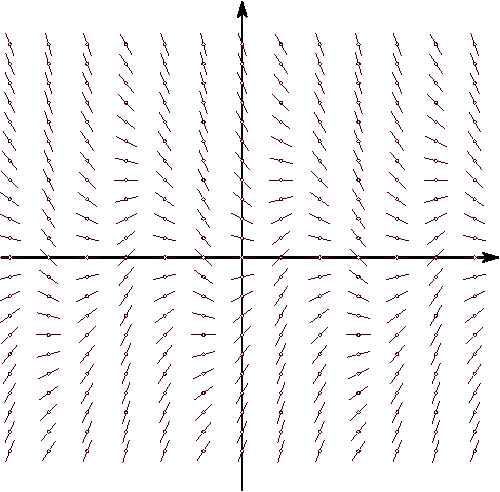
\includegraphics[width=0.45\textwidth]{03directionfield.pdf}\hfill
  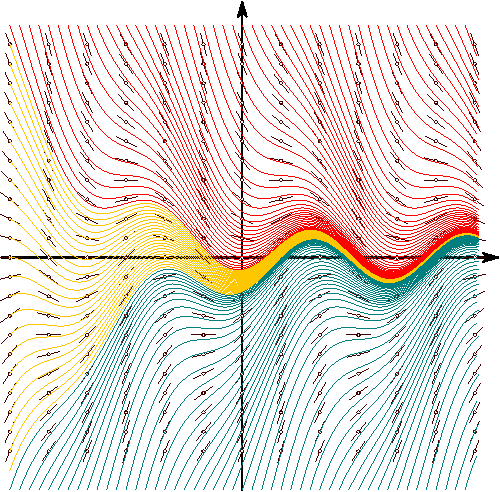
\includegraphics[width=0.45\textwidth]{03directionfield-withsolutions.pdf}
  \caption{Direction field for $\frac{\dd y}{\dd x} = -y+\sin\pi x$ on the left, and
    the same direction field with solutions to the differential equation.}
  \label{fig:direction-fields}
\end{figure}
It is clear from a quick look at Figure~\ref{fig:direction-fields} that drawing a
direction field involves computing $f(x,y)$ (i.e.~$-y+\sin\pi x$ in our example) for
\textit{many, many} points $(x, y)$.  This kind of repetitive computation is better
done by a computer, and an internet search quickly leads to a number of websites that
produce direction fields for our favorite differential equation.  In particular the
ODE page at the Virtual Math Museum of UC Irvine,
\begin{center}
  \url{http://virtualmathmuseum.org}
\end{center}
draws both direction fields and approximations to solutions found using Euler's
method, to which we now turn.


\section{Euler's method} %{{{1
\label{sec:eulers-method}
\subsection{The idea behind the method} %{{{2
Consider again the differential equation~\eqref{eq:mother-of-all-diffeqs},
\[
\frac{\dd y} {\dd x} = f(x, y).
\]
Suppose we know one point on a solution, i.e.~suppose we know that a given solution
to this equation satisfies $y=y_0$ when $x=x_0$, i.e.
\begin{equation}
  y(x_0) = y_0.
  \label{eq:initial-data}
\end{equation}
The differential equation then tells us what the derivative of the solution is at
$x=x_0$, namely,
\[
y'(x_0) = f(x_0, y_0).
\]
The definition a derivative says that
\[
y'(x_0) =\lim_{h\to 0} \frac{y(x_0+h) - y(x_0)} {h}
\]
so that we have
\begin{equation}
  \lim_{h\to 0} \frac{y(x_0+h) - y(x_0)} {h}  = f(x_0, y_0).
  \label{eq:diffeq-euler-derivation}
\end{equation}
Keep in mind that the right hand side is what we get by substituting the $x$ and $y$
values that we know for the solution in $f$.  So if we know $x_0$ and $y_0$ then we
can also compute $f(x_0, y_0)$.

If we don't know the solution then we cannot compute the left hand side in
\eqref{eq:diffeq-euler-derivation}, but, following Euler, we can make an
approximation.  If instead of letting $h\to0$ we choose a small number $h>0$, then we
may assume that
\begin{equation}
  \frac{y(x_0+h) - y(x_0)} {h}  \approx f(x_0, y_0).
  \label{eq:diffeq-euler-derivation2}
\end{equation}
Here ``$\approx$'' means ``approximately equal,'' which is a vaguely defined concept.
It means that the difference between the two quantities in
\eqref{eq:diffeq-euler-derivation2} is ``small'' and we will not worry too much about
the error in~\eqref{eq:diffeq-euler-derivation2} (such issues are addressed in more
advanced courses on Numerical Analysis; e.g.~Math 514 at UW Madison).
\begin{figure}
  \centering
  \problemfont% %{{{3
  \input ../figures/222/03diffeq-euler-one-step.pdf_tex
  \noproblemfont
  \hfill
  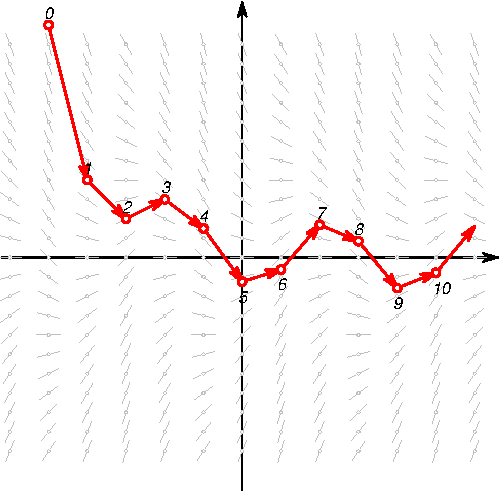
\includegraphics[width=0.5\textwidth]{03directionfield-euler.pdf}
  \caption{\textbf{Approximating a solution with Euler's method. } \textit{On the
      left}: one step of Euler's method.  Knowing one point $(x_0, y_0)$ on the graph
    does not immediately tell us what the solution is, but it does tell us what the
    tangent to the graph at $(x_0,y_0)$ is.  We can then guess that the point on the
    tangent with $x_1=x_0+h$ and $y_1=y_0+f(x_0, y_0)h$ \emph{almost} lies on the graph.\\
    ~\hspace{2em}\textit{On the right}: repeating the procedure gives us a sequence of points that
    approximate the solution.  Reducing the ``step size'' $h$ should give better
    approximations.}
  \label{fig:eulers-method}
\end{figure}
In the approximate equation~\eqref{eq:diffeq-euler-derivation2} all quantities are
known except $y(x_0+h)$.  After solving~\eqref{eq:diffeq-euler-derivation2} for
$y(x_0+h)$ we find
\[
  y(x_0+h) \approx y_0 + h f(x_0, y_0).
\]
Euler's idea (see Figure~\ref{fig:eulers-method}) was to forget that this is an
approximation, and declare that we now know a new point on the graph of the solution,
namely
\[
  x_1 = x_0+h, \qquad y_1 = y_0 + hf(x_0, y_0).
\]
Assuming that our solution satisfies $y(x_1) = y_1$ exactly (rather than just
approximately), we can apply the same procedure and get another new point on
the graph of our solution:
\[
x_2 = x_1+h, \qquad y_2 = y_1+hf(x_1,y_1).
\]
By repeating this procedure we can generate a whole list of points $(x_0, y_0)$,
$(x_1,y_1)$, $(x_2, y_2)$, $(x_3, y_3)$, etc\dots that lie approximately on the graph
of the solution passing through the given initial point $(x_0,y_0)$.

\subsection{Setting up the computation} %{{{2
\label{sec:euler-how-organize}
If we are given $x_{\rm start}$ and $y(x_{\rm start}) = y_{\rm start}$, and if we
want to find $y(x_{\rm end})$ for some $x_{\rm end}>x_{\rm start}$, then we can
decide to approximate $y(x_{\rm end})$ by applying $n$ steps of Euler's method.
Since each step advances $x$ by an amount $h$, application of Euler's method will
advance $x$ by $nh$ after $n$ steps.  Thus we want
\[
nh = x_{\rm end}-x_{\rm start}, \quad \text{i.e.} \quad
h = \frac{x_{\rm end} - x_{\rm start}} {n}.
\]
Starting with the known value of $y$ at $x_{\rm start}$ we then apply Euler's method
$n$ times by filling out a table of the following form:

\medskip
\begin{center}
  \begin{tabular}{lccc}
    \toprule
    $x_k$ & $y_k$ & $m_k = f(x_k,y_k)$ & $y_{k+1} = y_k+m_k\cdot h$\\
    \midrule
    $x_0=x_{\rm start}$ & $y_{\rm start}$ & $m_0$ & $y_1$ \\
    $x_1=x_0+ h$ & $y_1$ & $m_1$ & $y_2$\\
    $x_2=x_0+2h$ & $y_2$ & $m_2$ &$y_3$\\
    $x_3=x_0+3h$ & $y_3$ & $m_3$ &$y_4$\\
    \vdots &&& \vdots \\
    $x_{n-1}=x_0+(n-1)h$ & $y_{n-1}$ & $m_{n-1}$ & $y_n$\\
    $x_n = x_{\rm end}$ & $y_n$ &  &\\
    \bottomrule
  \end{tabular}
\end{center}
\medskip

The procedure is very mechanical and repetitive, and is best programmed on a
computer.

Once the table has been computed the values in the first two columns can be used to
graph the approximation to the real solution.

\section{Problems} %{{{1
\problemfont %{{{3
\begin{multicols}{2}


\problem Let  $y(t)$ be the solution of %{{{3
\[
  \frac{\dd y}{\dd t} = -t\cdot y, \quad y(1.0) = 10.0.
\]
We want to compute $y(3.0)$.

\subprob Find an exact formula for $y(3.0)$ by solving the equation (the equation is
both separable and linear, so we have at least two methods for finding the solution.)

\subprob If we use Euler's method with step size $h=2.0$, then how many steps do we
have to take to approximate $y(3.0)$?  Compute the approximation with $h=2.0$.

\subprob Find the approximations if $h=1.0$, $h=2/3$, and $h=0.5$.  Organize the
computations following the table in \ref{sec:euler-how-organize}.

\subprob Compare the results from the computations in \textbf{(b)} and \textbf{(c)}
with the true value of $y(3.0)$ from part \textbf{(a)}.

\problem \carefulnow  The function $y(x) = e^x$ is the solution to %{{{3
\[
  \frac{\dd y}{\dd x} = y, \quad y(0) = 1.
\]

\subprob Approximate $e=y(1)$ by using Euler's method first with step size $h=1$,
then with $h=1/2$, and then with $h=1/3$.  What are the approximations you find for
$y(1)$ in each case?

\subprob Look for a pattern in the answers to \textbf{(a)}.

\subprob Find a formula for the result of applying Euler's method $n$ times with
step size $h=\frac1n$. 

\problem Use Euler's method to approximate the solution to %{{{3
\[
\frac{\dd y} {\dd x} = -10 y,\quad y(0) = 1,
\]
and, in particular to find $y(1)$.  Use various step sizes.  How small do you have to
make the step size before the answer seems reasonable?  Explain.


\end{multicols}
\noproblemfont
\section{Applications of Differential Equations} %{{{1
\label{sec:diffeq-applications}
Differential equations are very often used to describe how some ``object'' or
``system'' changes or evolves in time.  If the object or system is simple enough then
its state is completely determined by one number (say $y$) that changes with time
$t$.

A differential equation for the system tells us how the system changes in time, by
specifying the rate of change of the state $y(t)$ of the system.  This rate of change
can depend on time, and it can depend on the state of the system, i.e.~on $y(t)$.
This dependence can be expressed as an equation of the form
\begin{equation}
  \label{eq:dynamics1}
  \frac{\dd y}{\dd t} = f(y, t).
\end{equation}
The function $f$ describes the \textit{evolutionary law} of our system (synonyms:
``evolutionary law'', ``dynamical law'', ``evolution equation for $y$'').

\subsection{Example: carbon dating} %{{{2
Suppose we have a fossil, and we want to know how old it is.

All living things contain carbon, which naturally occurs in two isotopes,
$\mathrm{C}_{14}$ (unstable) and $\mathrm{C}_{12}$ (stable). A long as the living
thing is alive it eats \& breaths, and its ratio of $\mathrm{C}_{12}$ to
$\mathrm{C}_{14}$ is kept constant.  Once the thing dies the isotope
$\mathrm{C}_{14}$ decays into $\mathrm{C}_{12}$ at a steady rate that is
proportional to the amount of $\mathrm{C}_{14}$ it contains.

Let $y(t)$ be the ratio of $\mathrm{C}_{14}$ to $\mathrm{C}_{12}$ at time $t$. The
law of radioactive decay says that there is a constant $k>0$ such that
\[
\frac{\dd y(t)}{\dd t} = -k y (t).
\]
Solve this differential equation (it is both separable and first order linear: either
method works) to find the general solution
\[
y (t; C) = Ce^{-kt}.
\]
After some lab work it is found that the current $\mathrm{C}_{14} /\mathrm{C}_{12}$
ratio of our fossil is $y_{\text{now}}$. Thus we have
\[
y_{\text{now}} = Ce^{-kt_{\text{now} }} \implies C= y_{\text{now}}e^{kt_{\text{now} }}.
\]
Therefore our fossil's $\mathrm{C}_{14} /\mathrm{C}_{12}$ ratio at any other time $t$
is/was
\[
y (t) = y_{\text{now}}e^{k (t_{\text{now}}-t)}.
\]
This allows us to compute the time at which the fossil died. At this time the
$\mathrm{C}_{14} / \mathrm{C}_{12}$ ratio must have been the common value in all
living things, which can be measured -- let's call it $y_{\text{life}}$. Then at the
time $t_{\text{demise}}$ when our fossil became a fossil we would have had
$y(t_{\text{demise}}) = y_{\text{life}}$. Hence the age of the fossil would be given
by
\[
y_{\text{life}} = y(t_{\text{demise}}) = y_{\text{now}}e^{k
  (t_{\text{now}}-t_{\text{demise}})} \implies\text{\fbox{$\DS
    t_{\text{now}}-t_{\text{demise}} = \frac1k \ln \frac{x_{\text{life} }}{
      x_{\text{now} }}$ }}
\]


\medskip

\subsection{Example: dating a leaky bucket} %{{{2
\label{ex:leakybucket}
A bucket is filled with water.  There is a hole in the bottom of the bucket so the
water streams out at a certain rate.

\smallskip

\begin{center}
  \begin{minipage}[c]{2.5in}
    \begin{tabbing}
      $h'(t)$ \= \hfill\kill
      $h(t)$ \> the height of water in the bucket \\
      $A$    \> area of cross section of bucket \\
      $a$    \> area of hole in the bucket \\
      $v$    \> velocity with which water goes through the hole. 
    \end{tabbing}
  \end{minipage}\quad
  \begin{minipage}[c]{1in}
    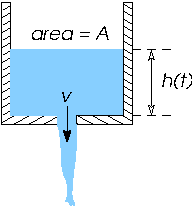
\includegraphics{04leakybucket.pdf}
  \end{minipage}
\end{center}
\noindent
We have the following facts to work with:
\begin{itemize}
\item  The amount (volume) of water in the bucket is $A\cdot h(t)$;
\item  The rate at which water is leaving the bucket is $a\cdot v(t)$;
\end{itemize}
Hence
\[
\frac{\dd Ah(t)}{\dd t} = - a v (t).
\]
In fluid mechanics it is shown that the velocity of the water as it passes through
the hole only depends on the height $h(t)$ of the water, and that, for some constant
$K$,
\[
v (t) = \sqrt{Kh(t)}.
\]
The last two equations together give a differential equation for $h (t)$, namely,
\[
\frac{\dd h(t)}{\dd t} = -\frac aA\sqrt{Kh(t)}.
\]
To make things a bit easier we assume that the constants are such that $\frac aA\sqrt
K=2$. Then $h (t)$ satisfies
\begin{equation}
  \label{eq:leaky-bucket}
  h'(t) = -2\sqrt{ h (t)}.
\end{equation}
This equation is separable, and when we solve it we get
\[
\frac{\dd h}{2\sqrt h} = - 1 \implies \sqrt{h(t)} = - t+C.
\]
This formula can't be valid for \textit{all} values of $t$, for if we take $t>C$, the
RHS becomes negative and can't be equal to the square root in the LHS. But when
$t\leq C$ we do get a solution,
\[
h (t;C) = (C-t)^2.
\]
This solution describes a bucket that is losing water until at time $C$ it is
empty. Motivated by the physical interpretation of our solution it is natural to
assume that the bucket stays empty when $t>C$, so that the solution with integration
constant $C$ is given by
\begin{equation}
  h(t) =
  \begin{cases}
    (C-t)^2 & \text{when }  t\leq C \\
    0 & \text{for } t>C.
  \end{cases}
  \label{eq:leaky-bucket-complete-solution}
\end{equation}
\begin{figure}
  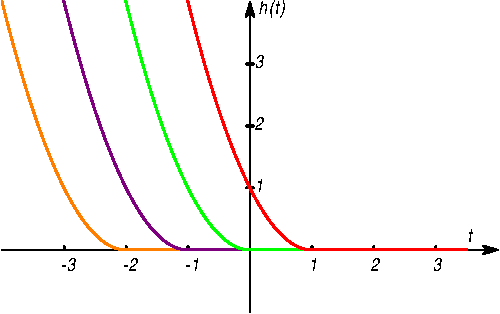
\includegraphics{04leakybucket-sltn.pdf}
  \caption{Several solutions $h (t; C)$ of the Leaking Bucket Equation
    (\ref{eq:leaky-bucket}).  Note how they all have the same values when $t\ge 1$.}
\end{figure}

\subsubsection*{The snag appears again} (See \S~\ref{sec:snag} and \S~\ref{ex:snag}.)
Note that we had to divide by $\sqrt{h}$ to find the solution.  This is not allowed
when $h=0$.  It turns out that $h(t) = 0$ is a solution to the differential equation.
The solution $h(t)=0$ satisfies $h(0)=0$, and our experience with differential
equations so far would lead us to believe that this should therefore be the only
solution that satisfies $h(0)=0$.  However, every solution
from~\eqref{eq:leaky-bucket-complete-solution} with $C\leq 0$ also satisfies
$h(0)=0$.  This problem is therefore different from the differential equations we
have dealt with up to now.  Namely, prescribing the value $y(0) = 0$ does not single
out one solution of the differential equation~\eqref{eq:leaky-bucket}.


 
\subsection{Heat transfer} %{{{2
\label{sec:diffeqs-heat-transfer}
We all know that heat flows from warm to cold: if we put a cold spoon in a hot cup of
coffee, then heat will flow from the coffee to the spoon.  How fast does the spoon
warm up?

According to physics the rate of change of the spoon's temperature is proportional to
the difference in temperature between the coffee and the spoon.  So, if $T_c$ and
$T_s$ are the temperature of the coffee and the spoon, respectively, then
\begin{equation}
  \frac{\dd T_s} {\dd t} = -K\bigl(T_s - T_c\bigr).
  \label{eq:Newtons-cooling-law}
\end{equation}
Here $K$ is a constant that depends on the shape and material of the spoon, how much
of the spoon is in the coffee, etc., but not on the temperatures $T_s$ and $T_c$.  If
we assume that the spoon is small, then whatever small amount of heat it extracts
from the coffee will not change the coffee temperature.  Under that assumption we may
assume that $T_c$ is a constant and the differential
equation~\eqref{eq:Newtons-cooling-law} is both separable and linear so that we have
two methods for solving it.

If the coffee itself is also cooling or warming up then $T_c$ will depend on time and
the equation~\eqref{eq:Newtons-cooling-law} becomes
\begin{equation}
  \label{eq:Newton-cooling-nonautonomous}
  \frac{\dd T_s} {\dd t} +K T_s = KT_c(t).
\end{equation}
If we know $T_c(t)$ then this is still a linear differential equation for $T_s$ and
we can solve it.

\subsection{Mixing problems} %{{{2
Consider a container containing water and vinegar.  If
water and vinegar are flowing in and out of the container, then the concentration of
vinegar in the container will change with time according to some differential
equation.  \textit{Which} differential equation describes the vinegar content of the
container depends on the precise details of the set-up.

As an example, let us assume that the container has fixed volume $V = 1000$ liters.
This means that the amount of liquid that flows in during any time interval must equal
the amount of liquid flowing out of the container (the liquid is ``incompressible,''
i.e.~its density is fixed.)

Suppose furthermore that a mixture of $5$\% vinegar and $95$\% water flows into the
container at $40$ liters per minute. And suppose also that the liquid in the
container is thoroughly mixed, so that the liquid that flows out of the container has
the same vinegar/water mixture as the entire container.

\marginpar{ 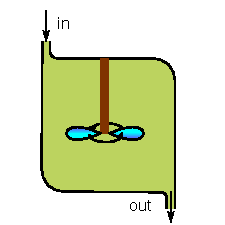
\includegraphics{03mixing.pdf}}




\subsubsection*{Problem:} Let $D(t)$ be the fraction of the liquid in the container
that is vinegar.  How does $D(t)$ change with time?

\subsubsection*{Solution:} Instead of tracking the concentration $D(t)$ of vinegar we
will look at the total amount of vinegar in the container.  This amount is $D(t)V$.

To find the differential equation we consider how much vinegar flows in and out of
the container during a short time interval of length $\Delta t$ (i.e.~between time
$t$ and $t+\Delta t$):
\begin{itemize}
\item [\textbf{in:}] The liquid volume flowing into the tank during a time $\Delta t$
  is $40\Delta t$ liters.  Since the vinegar concentration of the in-flowing liquid
  is $5$\%, this means that $5\%\cdot40\Delta t = 2\Delta t$ liters of vinegar
  enter the container.
\item [\textbf{out:}] Since $40\Delta t$ liters of liquid enter the container, the
  same amount of liquid must also leave the container.  The liquid that leaves is the
  well-stirred mixture, and thus it contains $D(t)\cdot40\Delta t $ liters vinegar.
\end{itemize}
In total we see that the change in vinegar content during a time $\Delta t$ is
\begin{equation}
\Delta\bigl(\text{vinegar content}\bigr) =
2 \Delta t - 40 D(t) \Delta t.
\label{eq:change-in-vinegar-content}
\end{equation}
To find the change in concentration we divide by the volume of the container
\[
\Delta D = \frac{2 \Delta t - 40 D(t) \Delta t} {1000} =
\frac{\Delta t} {500} - \frac{D(t)} {25} \Delta t.
\]
We find the rate of change by dividing by $\Delta t$ and letting $\Delta t\to0$:
\begin{equation}
  \frac{\dd D} {\dd t} = \frac{1} {500} - \frac{1} {25} D.
  \label{eq:diffeq-mixing-vinegar}
\end{equation}
This equation is again both linear and separable so we have two methods for solving
it.

\section{Problems} %{{{1
\problemfont %{{{3
\begin{multicols}{2}

\problem Read Example \ref{ex:leakybucket} on ``Leaky bucket dating'' %{{{3
again.  In that example we assumed that $\frac aA\sqrt K = 2$.

(a) Solve diffeq for $h(t)$ without assuming $\frac aA\sqrt K = 2$.
Abbreviate $C=\frac aA\sqrt K $.

(b) If in an experiment one found that the bucket empties in 20 seconds
after being filled to height $20$ cm, then how much is the constant
$C$?

\problem A population of bacteria grows at a rate proportional to its %{{{3
size. Write and solve a differential equation that expresses this. If
there are 1000 bacteria after one hour and 2000 bacteria after two hours,
how many bacteria are there after three hours?

\problem Rabbits in Madison have a birth rate of 5\% per year and a death %{{{3
rate (from old age) of 2\% per year. Each year 1000 rabbits get run over
and 700 rabbits move in from Sun Prairie.

\subprob Write a differential equation that describes Madison's rabbit
population at time $t$.
\answer %{{{3
Let $X(t)$ be the rabbit population size at time $t$.  The rate at which
this population grows is $dX/dt$ rabbits per year.
\begin{itemize}
\item [$\frac{5}{100}X$] from growth at 5\% per year
\item [$\frac{2}{100}X$] from death at 2\% per year
\item [$-1000$] car accidents
\item [$+700$] immigration from Sun Prairie
\end{itemize}
Together we get
\[
\frac{dX}{dt} = \frac{3}{100}X - 300.
\]
This equation is both separable and first order linear, so we can choose
from two methods to find the general solution, which is
\[
X(t) = 10,000 + C e^{0.03 t}.
\]
If $X(1991) = 12000$ then
\[
10,000 + C e^{0.03\cdot 1991} = 12,000 \implies C = 2,000e^{-0.03\cdot
1991} \text{(don't simplify yet!)}
\]
Hence
\[
X(1994) = 10,000 + 2,000e^{-0.03\cdot 1991}e^{0.03\cdot 1994} =10,000 +
2,000e^{0.03\cdot (1994-1991)} =10,000 + 2,000e^{0.09} \approx
12,188.\ldots
\]
\endanswer

\subprob If there were 12,000 rabbits in Madison in 1991, how many are
there in~1994?


\problem \groupproblem % Newton's cooling law, autonomous case %{{{3
Consider a cup of soup that is cooling by exchanging heat with the room.
If the temperature of the soup is $T_s(t)$, and if the temperature of the room is
$T_r$, then Newton's cooling law claims that
\[
\frac{\dd T_s} {\dd t} = -K (T_s- T_r)
\]
for some constant $K>0$.

\subprob What units does $K$ have, if we measure temperature in degrees Fahrenheit,
and time in seconds?
\answer %{{{3
$\sec^{-1}$.
\endanswer

\subprob Find the general solution to Newton's cooling law.  What units does the
arbitrary constant in your solution have?  What is the limit of
the temperature as $t\to\infty$?
\answer %{{{3
$T_s(t) = T_r + C e^{-Kt}$.  $C$ has the same units as $T_r$ and $T_s$, so $C$ is a
temperature:  degree Fahrenheit.  $\lim_{t\to\infty} T_s(t) = T_r$: in the long run
the soup will approach room temperature.
\endanswer

\subprob The soup starts at  $180^o$F, and sits in a room whose temperature is
$75^\circ$F.  In five minutes its temperature has dropped to $150^\circ$F.  Find the
cooling constant $K$.  When will its temperature be $90^\circ$F?
\answer %{{{3

(ii) Given $T_s(0) = 180$, $T_r=75$, and $T_s(5) = 150$. This gives the following
equations:
\[
T_r + C = 180, \quad T_r + Ce^{-5K} = 105
\implies C= 105, \quad -5K = \ln\frac{30}{105} =\ln\frac{2}{7}=-\ln\frac72.
\]
When is $T_s=90$?  Solve $T_s(t) = 90$ for $t$ using the values for $T_r$, $C$, $K$
found above ($K$ is a bit ugly so we substitute it at the end of the
problem):
\[
T_s(t) = T_r+Ce^{-Kt} = 75+105 e^{-Kt} = 90 \implies e^{-Kt} =
\frac{15}{105} = \frac{1}{7}.
\]
Hence
\[
t = \frac{\ln 1/7}{-K} = \frac{\ln 7}{K} = \frac{\ln 7}{\ln 7/2}.
\]

\endanswer

\problem \groupproblem A lake gets heated by day when the sun is out, and loses %{{{3
heat at night.  It also exchanges heat with the Earth.  The Earth's temperature
is $T_e$, and the lake's temperature is $T_l(t)$.  

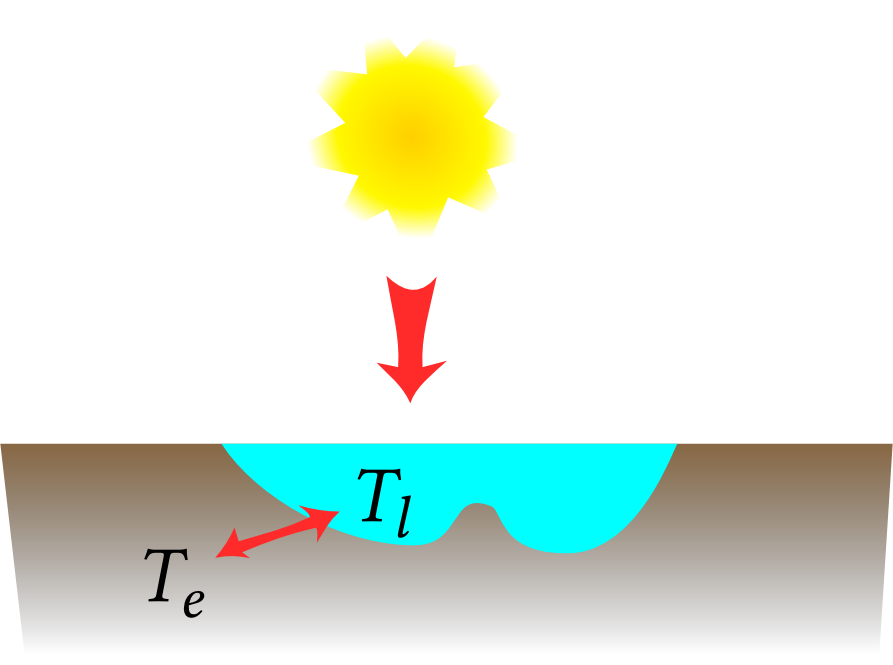
\includegraphics{03lakeandsun.png}

\noindent%
These effects together can be
modeled by a differential equation for $T_l(t)$
\[
\frac{\dd T_l} {\dd t}  = -K(T_l - T_e) + S \sin(2\pi t).
\]
Here the first term on the right represents Newton's cooling law, while the second
term accounts for the heating and cooling by radiation: if $\sin(2\pi t)>0$ then it's
day and the sun is heating the lake, if $\sin(2\pi t)<0$ then it's night and the lake
is radiating heat into the cold sky.  Time $t$ is measured in days. Temperatures are
in degrees Celsius.

\subprob Assuming $K=S=1$, and $T_e=10$ find the general solution to the differential
equation.

\subprob Draw the direction field for the differential equation when $K=S=1$ and $T_e
= 10$.  (First try to do this by hand.  Then use a computer.)

\subprob Does $\lim_{t\to\infty} T_l(t)$ exist?  Consider the separate terms in the
general solution you found in part \textbf{(a)}, and see if any of these terms have a
limit as $t\to\infty$.

\subprob Find the solution for arbitrary $K$ and $S$ (you may assume $K$ and $S$ are
positive.)


\problem Retaw is a mysterious living liquid; it grows at a rate of $5\%$ of its %{{{3
volume per hour.  A scientist has a tank initially holding $y_0$ gallons of
retaw and removes retaw from the tank continuously at the rate of 3 gallons per
hour.
\answer %{{{3
(a) Let $y(t)$ be the amount of ``retaw'' (in gallons) in the tank at time
$t$.  Then
\[
\frac{dy}{dt} = \underbrace{\frac{5}{100}y}_{\rm growth}
- \underbrace{\quad3\quad}_{\rm removal}.
\]
(b) $y(t) = 60+ Ce^{t/20} = 60+(y_0 - 60)e^{t/20}$.

(c) If $y_0 = 100$ then $y(t) = 60 + 40 e^{t/20}$ so that
$\lim_{t\to\infty} y(t) = +\infty$.

(d) $y_0 = 60$.
\endanswer

\subprob Find a differential equation for the number $y(t)$ of gallons of
retaw in the tank at time $t$.

\subprob Solve this equation for $y$ as a function of $t$. (The initial
volume $y_0$ will appear in our answer.)

\subprob What is $\lim_{t\to\infty} y(t)$ if $y_0=100$?

\subprob What should the value of $y_0$ be so that $y(t)$ remains constant?


\problem A 1000 gallon vat is full of 25\% solution of acid. Starting at %{{{3
time $t=0$ a 40\% solution of acid is pumped into the vat at 20 gallons per
minute. The solution is kept well mixed and drawn off at 20 gallons per
minute so as to maintain the total value of 1000 gallons. Derive an
expression for the acid concentration at times $t>0$. As $t\to\infty$ what
percentage solution is approached?
\answer %{{{3
Finding the equation is the hard part.  Let $A(t)$ be the 
\emph{volume} of acid in the vat at time $t$.  Then $A(0) = 25\%\text{ of
}1000 = 250$gallons.

$A'(t) = $ the volume of acid that gets pumped in minus the volume that gets
extracted per minute.  Per minute $40\%$ of $20$ gallons, i.e.\ 8 gallons of
acid get added.  The vat is well mixed, and $A(t)$ out of the $1000$gallons
are acid, so if 20 gallons get extracted, then $\frac{A}{1000}\cdot20$ of
those are acid.  Hence
\[
\frac{dA}{dt} = 8 - \frac{A}{1000}\cdot20 = 8-\frac{A}{50}.
\]
The solution is $A(t) = 400 + Ce^{-t/50} = 400 + (A(0)-400)e^{-t/50} = 400
-150 e^{-t/50}$.

The \emph{concentration} at time $t$ is 
\[
\text{concentration} = \frac{A(t)}{\text{total volume}} = 
\frac{400 - 150e^{-t/50}}{1000} = 0.4 - 0.15 r^{-t/50}.
\]
If we wait for very long the concentration becomes
\[
\text{concentration} = \lim_{t\to\infty} \frac{A(t)}{1000} = 0.4.
\]
\endanswer

\problem [\textbf{Mixing}] The volume of a lake is $V=10^9$ cubic feet.  Pollution $P$ runs %{{{3
into the lake at $3$ cubic feet per minute, and clean water runs in at $21$
cubic feet per minute.  The lake drains at a rate of $24$ cubic feet per
minute so its volume is constant. Let $C$ be the concentration of pollution
in the lake; i.e. $C=P/V$.

\subprob Give a differential equation for $C$.

\subprob Solve the differential equation. Use the initial condition $C=C_0$
when $t=0$ to evaluate the constant of integration.

\subprob There is a critical value $C^*$ with the property that for any
solution $C=C(t)$ we have
\[
\lim_{t\to\infty}C= C^*.
\]
Find $C^*$. If $C_0=C^*$, what is $C(t)$?
\answer %{{{3
$P$ is the volume of polluted water in the lake at time $t$.
At any time the fraction of the lake water that is polluted is $P/V$, so if
24 cubic feet are drained then $\frac{P}{V}\cdot24$ of those are polluted.
Here $V=10^9$; for simplicity we'll just write $V$ until the end of the
problem. We get
\[
\frac{dP}{dt} = \text{"in minus out"}
= 3 - \frac{P}{V} \cdot 24
\]
whose solution is $P(t) = \frac{1}{8}V+Ke^{-\frac{24}{V}t}$.  Here
$K$ is an arbitrary constant (which we can't call $C$ because in this
problem $C$ is the concentration).

The concentration at time $t$ is 
\[
C(t) = \frac{P(t)}{V} = \frac18 + \frac{K}{V}e^{-\frac{24}{V}t} 
=\frac18 + \bigl(C_0 - \frac18\bigr) e^{-\frac{24}{V}t} .
\]
No matter what $C_0$ is we always have
\[
\lim_{t\to\infty} C(t) = 0
\]
because $\lim_{t\to\infty} e^{-\frac{24}{V}t} = 0$.

If $C_0 = \frac18$ then the concentration of polluted water remains
constant: $C(t) = \frac18$.
\endanswer

\problem [\textbf{Mixing}] A 300 gallon tank is full of milk containing 2\% %{{{3
butterfat.  Milk containing 1\% butterfat is pumped in a 10 gallons per minute
starting at 10:00 AM and the well mixed milk is drained off at 15 gallons per minute.
What is the percent butterfat in the milk in the tank 5 minutes later at 10:05 AM?
Hint: How much milk is in the tank at time $t$?  How much butterfat is in the milk at
time $t=0$?



\problem \groupproblem A philanthropist endows a chair. This means that she %{{{3
donates an amount of money $B_0$ to the university.  The university invests
the money (it earns interest) and pays the salary of a professor.  Denote
the interest rate on the investment by $r$ (e.g. if $r=.06$, then the
investment earns interest at a rate of $6\%$ per year) the salary of the
professor by $a$ (e.g. $a=\$50,000$ per year), and the balance in the
investment account at time $t$ by $B$.

\subprob Give a differential equation for $B$.

\subprob Solve the differential equation. Use the initial condition $B=B_0$
when $t=0$ to evaluate the constant of integration.

\subprob There is a critical value $B^*$ with the property that (1)~if
$B_0<B^*$, then there is a $t>0$ with $B(t)=0$ (i.e. the account runs out
of money) while (2)~if $B_0>B^*$, then $\lim_{t\to\infty}B=\infty$.  Find
$B^*$.

\subprob This problem is like the pollution problem except for the signs of
$r$ and $a$. Explain.

\problem \groupproblem A citizen pays social security taxes of $a$ dollars %{{{3
per year for $T_1$ years, then retires, then receives payments of $b$
dollars per year for $T_2$ years, then dies. The account which receives and
dispenses the money earns interest at a rate of $r$\% per year and has no
money at time $t=0$ and no money at the time $t=T_1+T_2$ of death.  Find
two differential equations for the balance $B(t)$ at time $t$; one valid
for $0\le t\le T_1$, the other valid for $T_1\le t\le T_1+T_2$.  Express
the ratio $b/a$ in terms of $T_1$, $T_2$, and $r$.  Reasonable values for
$T_1$, $T_2$, and $r$ are $T_1=40$, $T_2=20$, and $r=5\%=.05$. This model
ignores inflation. Notice that $0<dB/\dd t$ for $0<t<T_1$, that $dB/\dd
t<0$ for $T_1<t<T_1+T_2$, and that the account earns interest {\em even for
} $T_1<t<T_1+T_2$.


\end{multicols}
\noproblemfont


%%% Local Variables: 
%%% mode: latex
%%% TeX-master: "free222"
%%% End: 
